
%(BEGIN_QUESTION)
% Copyright 2015, Tony R. Kuphaldt, released under the Creative Commons Attribution License (v 1.0)
% This means you may do almost anything with this work of mine, so long as you give me proper credit

Determine what these two voltmeters will register with the circuit grounded at three different points (each grounding scenario considered one at a time, not simultaneously).  Note that neither voltmeter moves, nor are any of their test leads moved, between scenarios.  The only difference is where we connect earth ground to the circuit:

$$\includegraphics[width=15.5cm]{i03649x01.eps}$$

% No blank lines allowed between lines of an \halign structure!
% I use comments (%) instead, so that TeX doesn't choke.

$$\vbox{\offinterlineskip
\halign{\strut
\vrule \quad\hfil # \ \hfil & 
\vrule \quad\hfil # \ \hfil & 
\vrule \quad\hfil # \ \hfil \vrule \cr
\noalign{\hrule}
%
% First row
{\bf Grounded at:} & {\bf VM \#1} & {\bf VM \#2} \cr
%
\noalign{\hrule}
%
% Another row
Point A only &  &  \cr
%
\noalign{\hrule}
%
% Another row
Point B only &  &  \cr
%
\noalign{\hrule}
%
% Another row
Point C only &  &  \cr
%
\noalign{\hrule}
} % End of \halign 
}$$ % End of \vbox

\vskip 20pt \vbox{\hrule \hbox{\strut \vrule{} {\bf Suggestions for Socratic discussion} \vrule} \hrule}

\begin{itemize}
\item{} FOUNDATION Fieldbus H1 networks are floating (neither conductor grounded).  Given this fact, explain how voltmeter measurements might be useful in determining the existence of a grounded H1 segment conductor.
\item{} What would happen if points A and B were simultaneously grounded?  How about points B and C?  How about points A and C?
\end{itemize}

\underbar{file i03649}
%(END_QUESTION)





%(BEGIN_ANSWER)


%(END_ANSWER)





%(BEGIN_NOTES)

% No blank lines allowed between lines of an \halign structure!
% I use comments (%) instead, so that TeX doesn't choke.

$$\vbox{\offinterlineskip
\halign{\strut
\vrule \quad\hfil # \ \hfil & 
\vrule \quad\hfil # \ \hfil & 
\vrule \quad\hfil # \ \hfil \vrule \cr
\noalign{\hrule}
%
% First row
{\bf Grounded at:} & {\bf VM \#1} & {\bf VM \#2} \cr
%
\noalign{\hrule}
%
% Another row
Point A only & 18 volts & 18 volts \cr
%
\noalign{\hrule}
%
% Another row
Point B only & 18 volts & 10 volts \cr
%
\noalign{\hrule}
%
% Another row
Point C only & 18 volts & 0 volts \cr
%
\noalign{\hrule}
} % End of \halign 
}$$ % End of \vbox


%INDEX% Electronics review: Kirchhoff's Voltage Law (KVL)

%(END_NOTES)


